% ---------------------------------------------------------------------------
% Cosyne 2027 two-page extended abstract (deadline 18 October 2026).
%
% Format rules (cosyne.org/abstracts-submission, read 8 Oct 2026):
%   * two-page PDF, US Letter or A4, margins >= 0.5 in
%   * body font >= 12 pt; figure captions and references may be 10 pt
%   * title <= 100 characters incl. spaces, sentence case
%   * a <= 300-word summary (also pasted into a text-only box on the
%     submission site; it is the only text published in the program and
%     cannot be revised afterwards) followed by "additional detail"
%     (question, approach, results, conclusions; figures and equations
%     encouraged).  Reviewers see only this PDF.
%   * double blind: no names, affiliations, acknowledgments, or author
%     metadata; cite our own work in the third person ("[1]").
%   * pages beyond two are removed; non-compliant PDFs may be desk-rejected.
% There is no official template.  This file is self-contained and compiles
% with pdfLaTeX (no BibTeX needed: the reference list is written by hand).
%
% Figure plan.  Both figures are STAND-INS (paper figures squeezed into a
% dashed box of the intended footprint); remake offline at the stated size.
%   Fig 1 (full width x 1.7 in)
%     A  closed-loop paradigm: fit encoding model -> accentuate -> present
%     B  neural: (i) matched held-out prediction, (ii) two models' images
%        from one seed, (iii) self vs peer-review slope / R^2
%     C  linear teacher-student recapitulation of (i)-(iii)
%     D  equal-error geometry in the (high-PC, low-PC) weight plane:
%        prediction ellipsoids, control spheres, peer hyperplane, ridge path
%   Fig 2 (full width x 1.5 in)
%     A  pixel ridge on van Hateren: R^2_gen and R^2_acc vs kappa at 3-4
%        noise levels, DE lines + MC markers (or paper Fig. 3F)
%     B  gauge rotation of the top-500-PC map: E_gen flat, R^2_acc collapses
%     C  neural: site-centred control slope vs log10 V_phi scatter (r=-0.56)
%        + bar of -r for held-out MSE vs T_phi / V_phi across model subsets
% ---------------------------------------------------------------------------
\documentclass[12pt,letterpaper]{article}
\usepackage[margin=0.55in]{geometry}
\usepackage[T1]{fontenc}
\usepackage{times}
\usepackage{amsmath,amssymb,bm}
\usepackage{graphicx}
\usepackage{caption}
\usepackage[hidelinks]{hyperref}
\hypersetup{pdftitle={When good brain predictors make bad brain controllers: a regression theory of neural control},
            pdfauthor={},pdfsubject={Cosyne 2027 abstract},pdfkeywords={}}

\pagestyle{empty}
\setlength{\parindent}{0pt}
\setlength{\parskip}{1.5pt plus 1pt minus 1pt}
\linespread{0.87}
\setlength{\abovedisplayskip}{3pt}\setlength{\belowdisplayskip}{3pt}
\setlength{\abovedisplayshortskip}{2pt}\setlength{\belowdisplayshortskip}{2pt}
\captionsetup{font=footnotesize,labelfont=bf,labelsep=period,skip=2pt}  % footnotesize = 10 pt at 12 pt base
\setlength{\textfloatsep}{5pt}\setlength{\intextsep}{5pt}
% run-in bold headings
% (needspace-style guard so a heading is not stranded at a page bottom)
\newcommand{\runsection}[1]{\par\vskip0pt plus 3\baselineskip\penalty-100\vskip0pt plus -3\baselineskip\vspace{1.5pt}\noindent\textbf{#1}\hspace{0.5em}\ignorespaces}
% stand-in figure box: fixed footprint, dashed frame
\newcommand{\standin}[2]{\setlength{\fboxsep}{1pt}\setlength{\fboxrule}{0.3pt}%
  \fbox{\parbox[c][#1][c]{\dimexpr\linewidth-2\fboxsep-2\fboxrule}{\centering#2}}}
% non-floating figure: \placefig{height}{content}{caption}{label}
\newcommand{\placefig}[4]{\par\vspace{4pt}\noindent\begin{minipage}{\linewidth}\centering
  \standin{#1}{#2}\captionof{figure}{#3}\label{#4}\end{minipage}\par\vspace{4pt}}
% math
\newcommand{\x}{\mathbf{x}}
\newcommand{\bhat}{\hat{\beta}}
\newcommand{\bstar}{{\beta^{\star}}}
\newcommand{\bprime}{{\beta^{\prime}}}
\newcommand{\uvec}{\mathbf{u}}
\newcommand{\E}{\mathbb{E}}
\newcommand{\R}{\mathbb{R}}

\begin{document}

{\large\bfseries When good brain predictors make bad brain controllers: a regression theory of neural control\par}
\vspace{2pt}

% ---------------------------------------------------------------- summary (<= 300 words)
\textbf{Summary.}
Deep-network encoding models now predict the responses of visual cortical neurons to natural images so well that benchmarks can hardly rank them. The same models are increasingly used as controllers that synthesize images to drive a neuron to a target response. A recent closed-loop benchmark of ten encoding models at 25 macaque V4/IT sites~[1] found a striking dissociation. Models with nearly identical held-out accuracy generated visibly different images and differed several-fold in how well those images moved the neuron; models that failed to control still recognized the successful images of other models; and control success tracked the spatial-frequency content of a model's input gradient rather than its accuracy. We show that all three phenomena arise already in linear ridge regression, from a single fact: control evaluates a model on a distribution the model generates itself. Held-out prediction measures weight error in the metric of the natural-image covariance, which suppresses low-variance directions; a gradient-ascent path moves along the fitted weight and measures the same error in Euclidean geometry. Deterministic equivalents for ridge regression show that prediction-optimal and control-optimal regularization obey different spectral conditions, so cross-validation leaves a residual control error that grows with response noise. For models built on fixed feature maps, we construct families of maps with identical prediction but arbitrarily different control and isolate a gradient-geometry factor of the map alone that determines when control is fragile. A Jacobian version of this factor ranks deep encoding models by \emph{in vivo} control across 250 site--model pairs, where held-out accuracy carries no information. Predictivity benchmarks therefore cannot certify a model for control; its gradients or generated stimuli must be tested directly.

% ---------------------------------------------------------------- additional detail
\runsection{The phenomena.}
In the closed-loop paradigm of~[1] (Fig.~1A), responses of 25 V3/V4--IT sites in five macaques to ${\sim}1000$ naturalistic images were fit by cross-validated ridge regression on the features of ten deep-network backbones; each model then synthesized images by feature accentuation~[2] to drive its own prediction to graded targets, which were tested in a second session. Three observations motivate the theory (Fig.~1B). (i)~Models tightly matched on held-out images differed widely in the slope and $R^2$ between predicted and measured responses to their own images, often reaching the target with high-frequency texture that left the neuron unmoved. (ii)~In ``peer review'', a model whose own images failed still predicted responses to a successful model's images, often better than the generator. (iii)~Models whose input gradients concentrate power at low spatial frequencies controlled best. A linear teacher--student model on natural images reproduces (i)--(iii) once the student's weight error lies along low-variance image directions (Fig.~1C).

\placefig{1.7in}{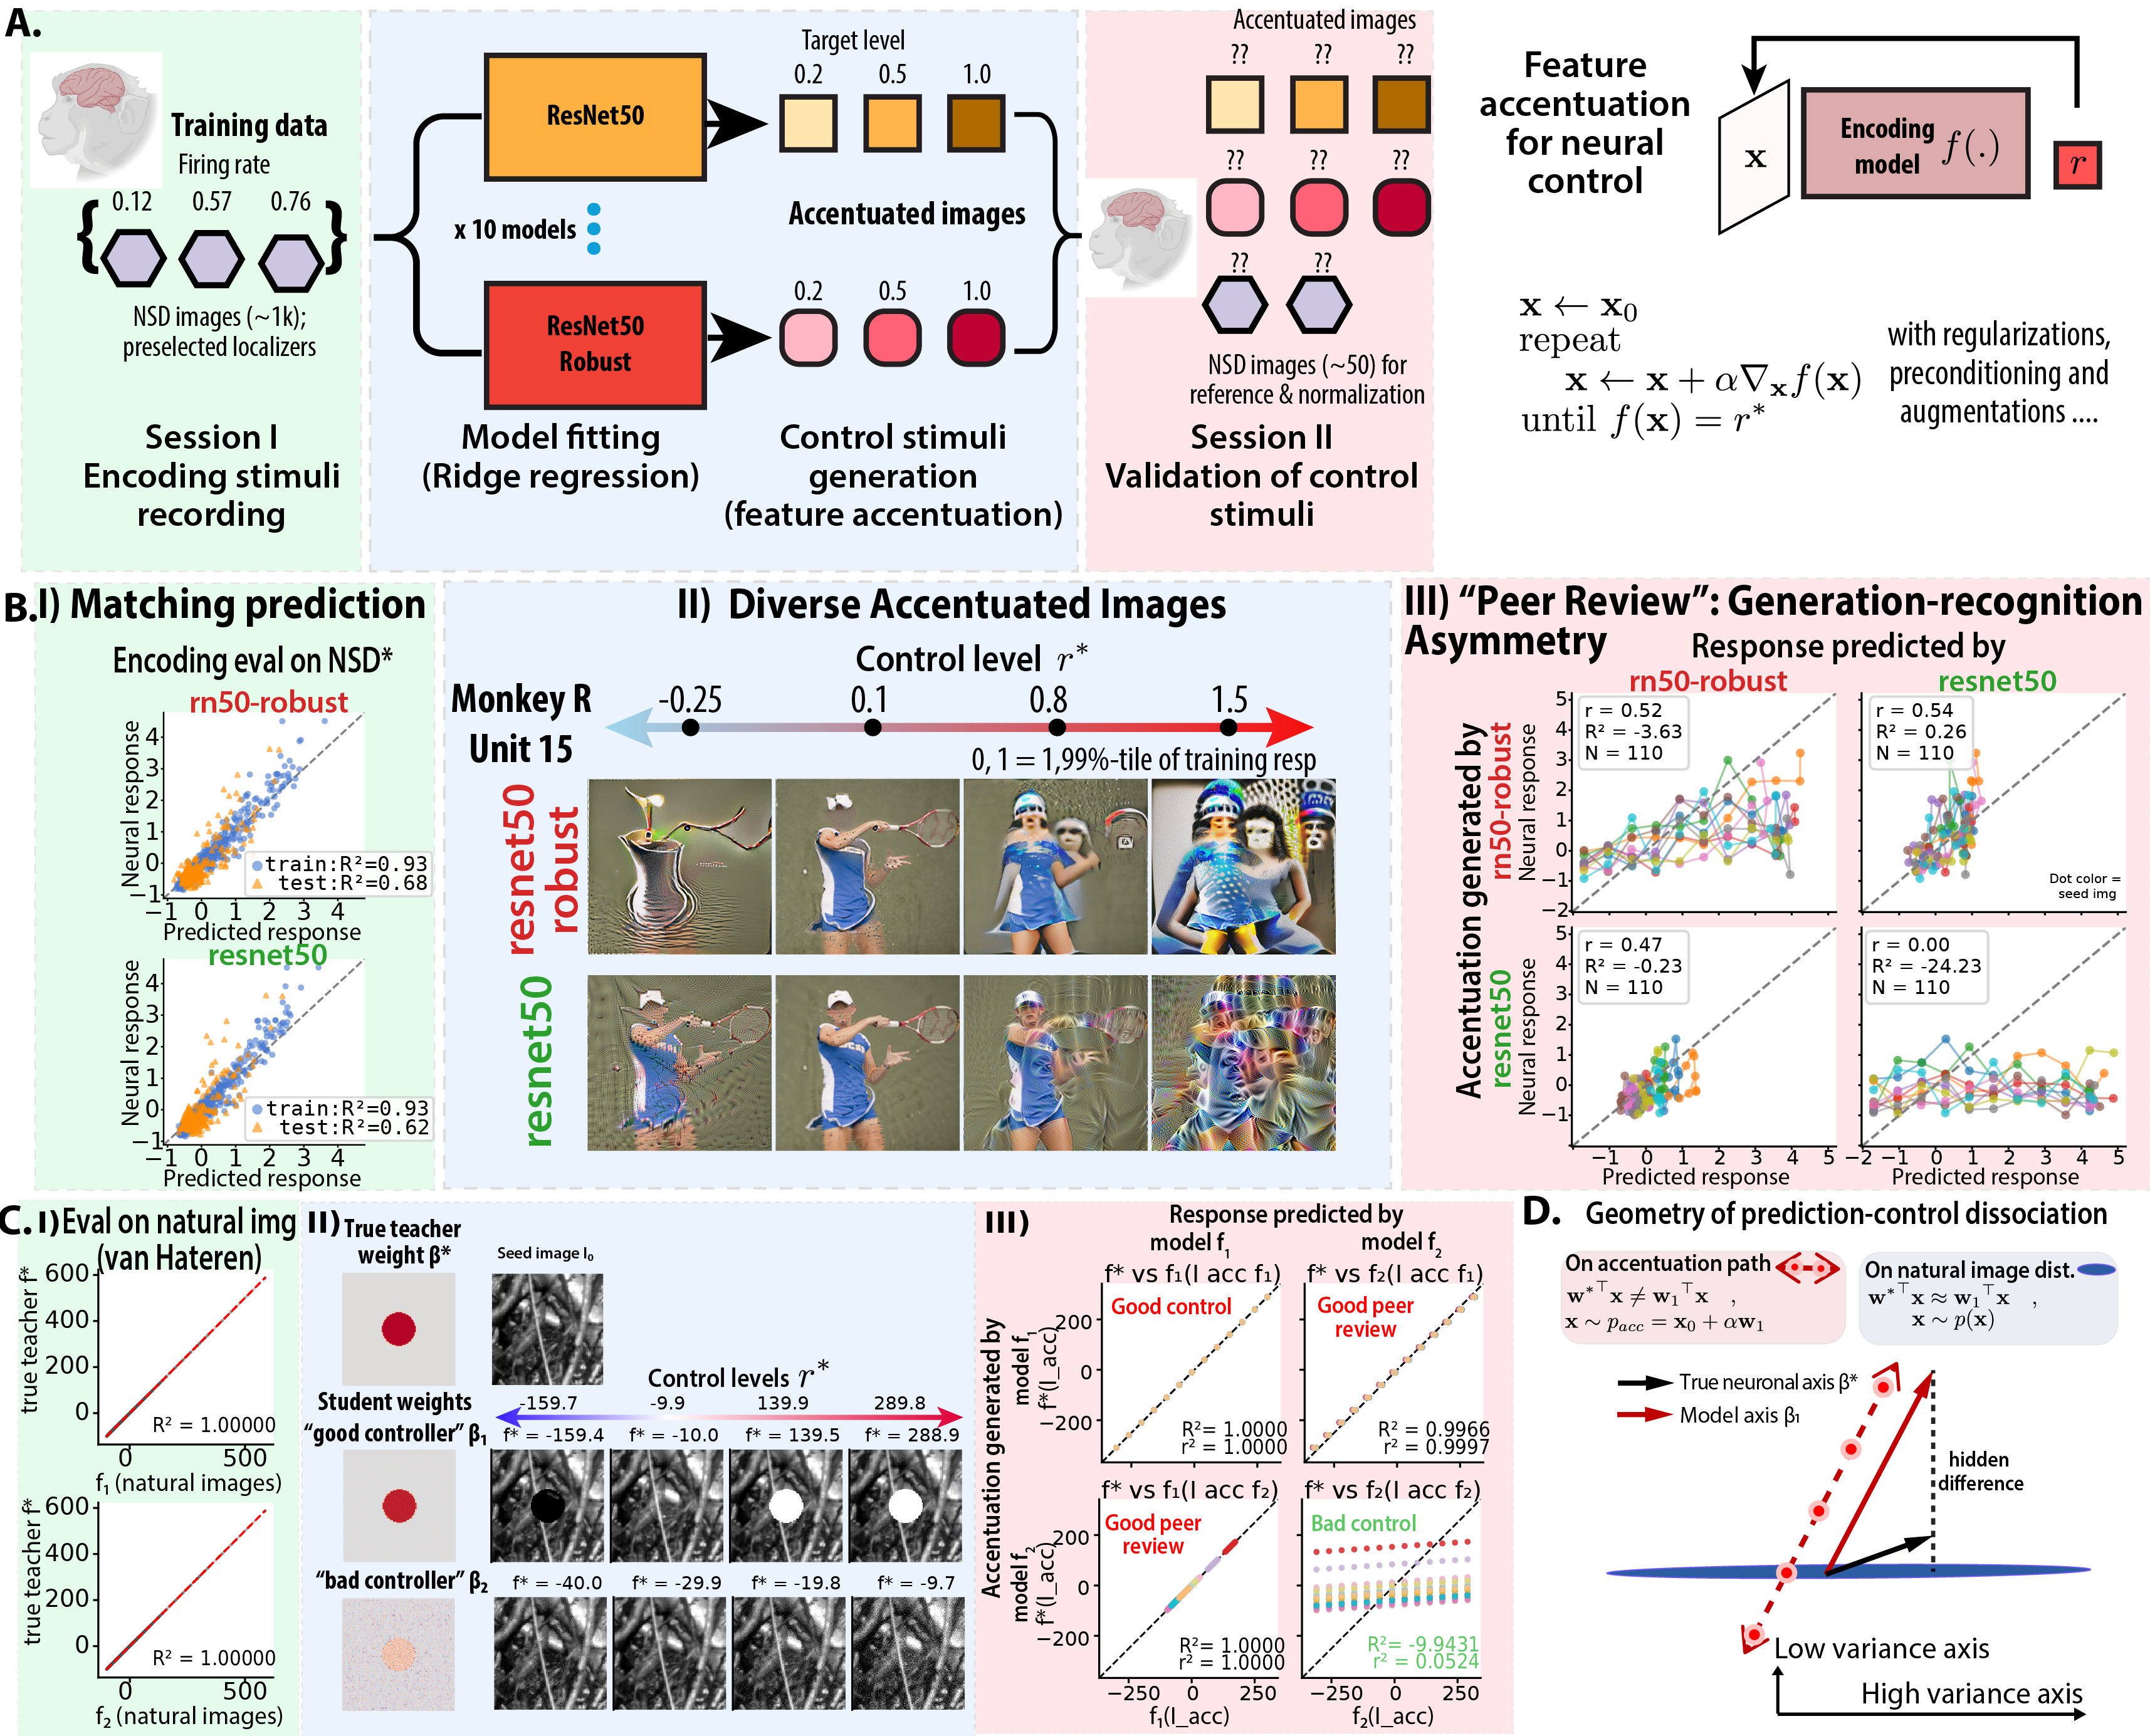
\includegraphics[height=1.65in]{figures/Figure_NeuroCtrl_results_Neuro-linear-compose.png}\hfill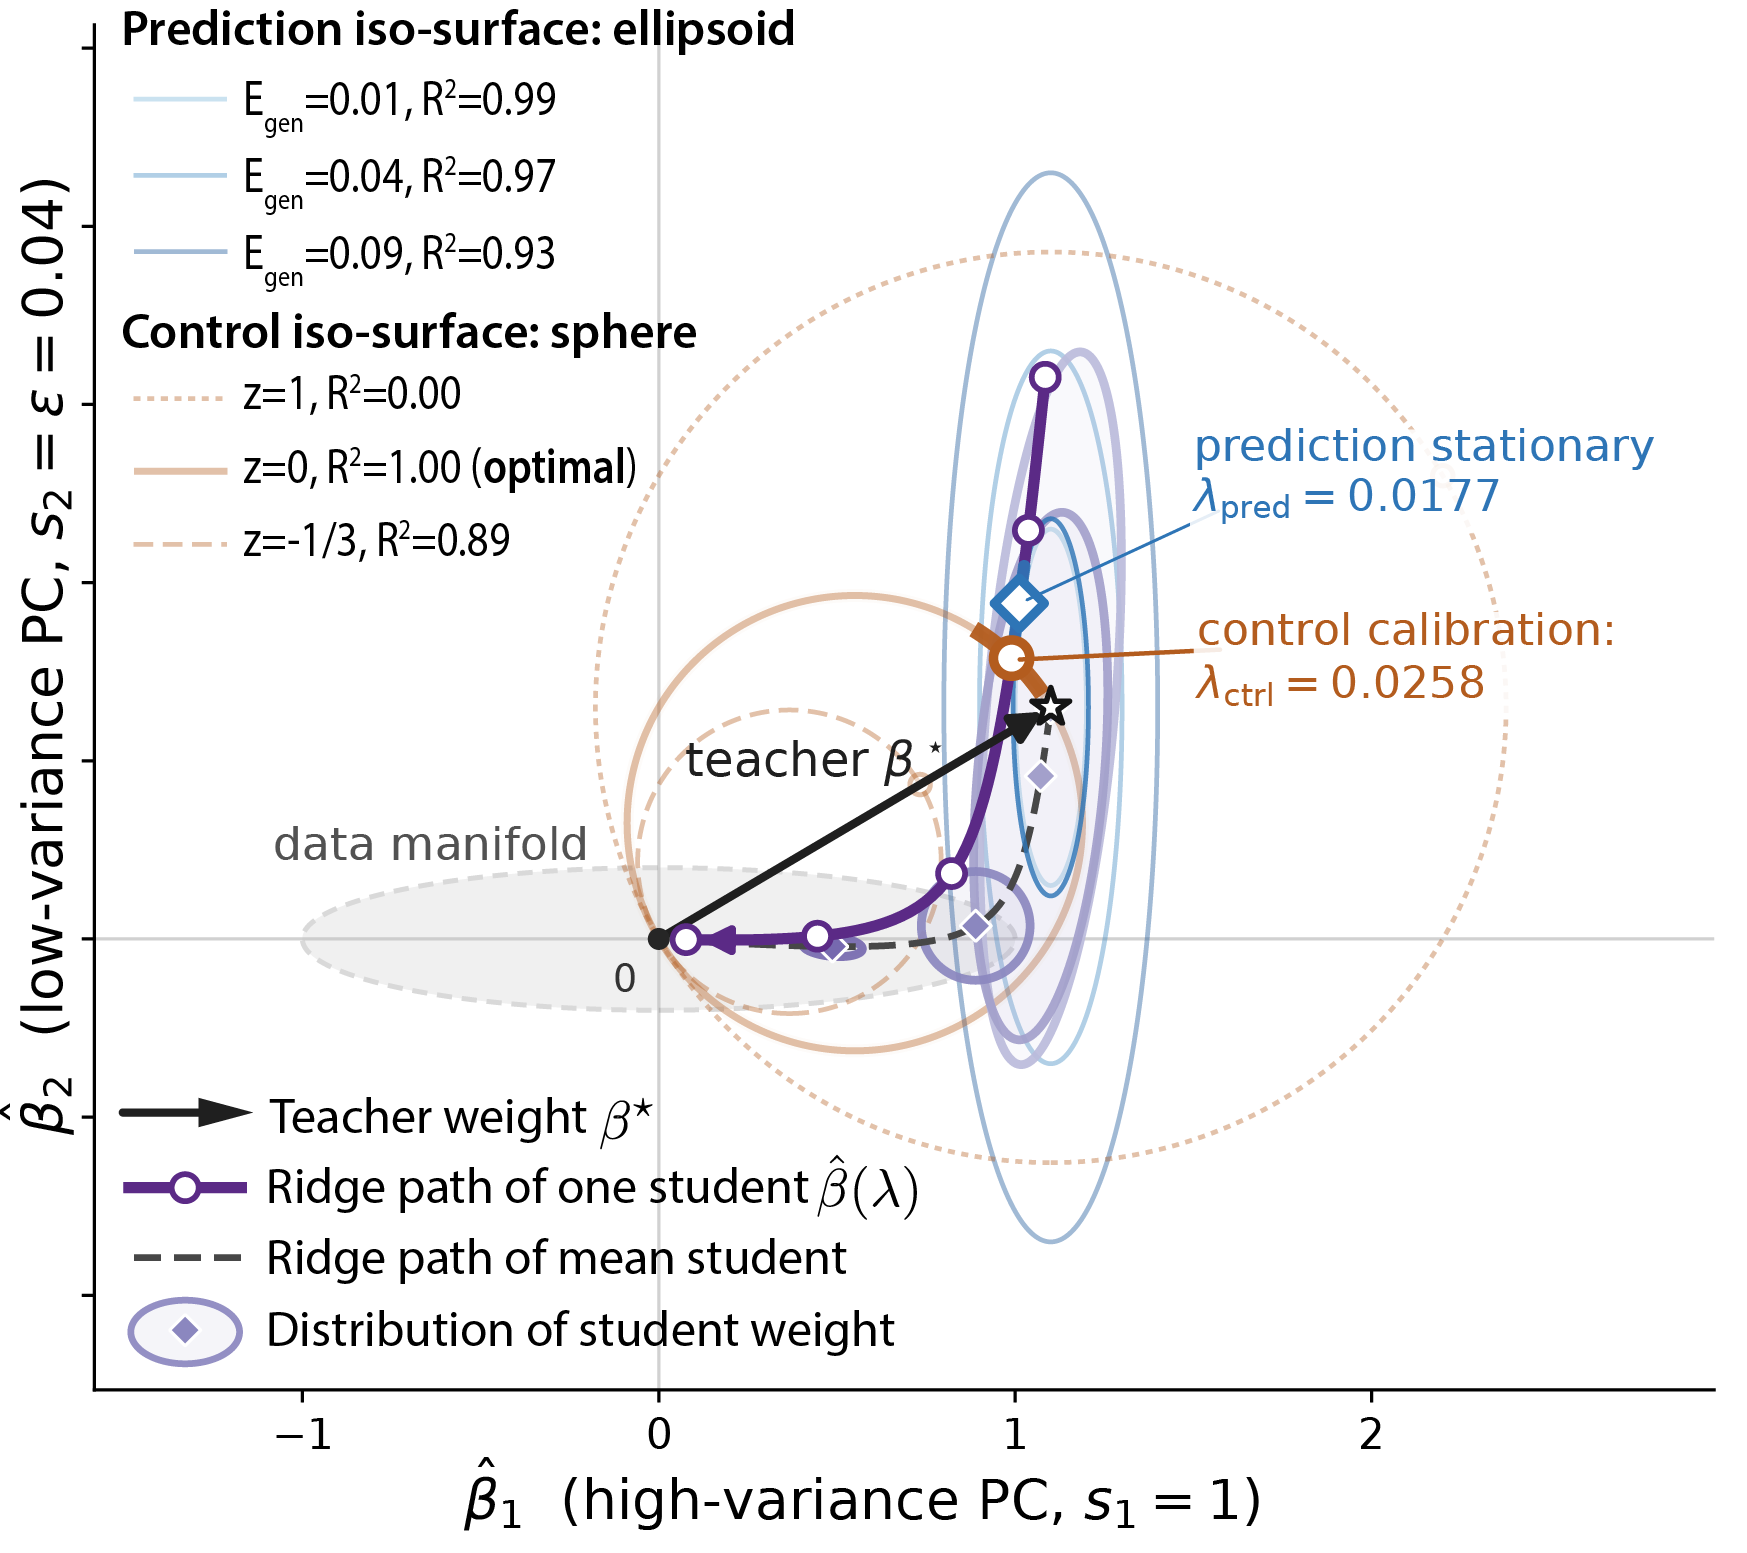
\includegraphics[height=1.65in]{figures/Figure_iso_err_surf_dissociation-01.png}}{\textbf{Prediction and control dissociate in neurons and in linear regression.}
\textbf{A}~Closed-loop paradigm of~[1]: encoding models fit to natural-image responses synthesize accentuated images that are tested in a second session.
\textbf{B}~Two models predict held-out responses equally well (i), generate different images from one seed (ii), and differ in self- versus peer-evaluated control (iii).
\textbf{C}~Two linear students of one linear teacher, differing only along low-variance image directions, reproduce (i)--(iii).
\textbf{D}~Equal-error sets in the plane of a high- and a low-variance principal component: prediction ellipsoids, control spheres and the ridge path $\bhat(\lambda)$.}{fig:phenomena}

\runsection{One predictor, three evaluation distributions.}
Let $\x\sim\mathcal N(0,\Sigma)$ with $\Sigma=\sum_k s_k\uvec_k\uvec_k^\top$, the neuron a noisy linear teacher $y=\x^\top\bstar+\sigma\epsilon$, and the model a student $f(\x)=\x^\top\bhat$ fit from $n$ pairs. Generalization evaluates $f$ on fresh natural inputs, accentuation on its own path $\x=\alpha\bhat$, and peer review on a peer's path $\x=\alpha\bprime$. With $\Delta=\bhat-\bstar$, $N=\bhat^\top\bstar$ and $D=\|\bhat\|^2$, generalization error is $E_{\rm gen}=\Delta^\top\Sigma\Delta$, whereas every accentuation metric is a function of $z:=D/N-1$: $\mathrm{slope}_{\rm acc}=1/(1+z)$ and $R^2_{\rm acc}=1-z^2$. Prediction weighs an error along $\uvec_k$ by $s_k$, so errors in low-variance directions are nearly invisible; control measures the same error in Euclidean geometry. The equal-error sets in weight space are ellipsoids elongated along low-variance axes, Euclidean spheres on the diameter from $0$ to $(1+z)\bstar$, and hyperplanes normal to $\bprime$ (Fig.~1D). The bad controller of Fig.~1C sits inside a small ellipsoid yet on a huge sphere, and on the zero-error hyperplane of the good one.

\runsection{Pixel-space ridge: noise, spectrum and regularization.}
Deterministic equivalents in the proportional limit $d/n\to\gamma$~[3,4] replace the empirical covariance by $\Sigma$ at an effective penalty $\kappa(\lambda)\ge\lambda$. With $B_{p,q}=\sum_k s_k^p b_k^2/(s_k+\kappa)^q$, $\mathrm{df}_{p,q}=\sum_k s_k^p/(s_k+\kappa)^q$ and $b_k=\uvec_k^\top\bstar$,
\begin{equation}\small
N\asymp B_{1,1},\qquad
D\asymp B_{2,2}+V,\qquad
V=\frac{\mathrm{df}_{1,2}}{n}\big(E_{\rm gen}+\sigma^2\big),
\qquad \|\bstar\|^2\ge B_{1,1}\ge B_{2,2}.
\label{eq:de}
\end{equation}
The mean fitted weight, the teacher shrunk mode by mode, \emph{under}-shoots its own path ($D<N$); the \emph{norm inflation} $V$, the Euclidean energy of the fit's noise part, enlarges $D$ but not $N$, so the student \emph{over}-predicts, and $R^2_{\rm acc}$ turns negative once $V$ exceeds the shrinkage deficit. Prediction-optimal and control-optimal penalties both equate $E_{\rm gen}+\sigma^2$ to $n\kappa$ times a spectral average of the teacher power $b_k^2$, but over bands centred at $s_k\approx2\kappa$ and $s_k\approx\kappa$; their mismatch is the control error left by cross-validation, which vanishes only for isotropic data or a spectrally flat teacher. On van Hateren images ($d=10^4$, $n=10^3$), along the cross-validated path $R^2_{\rm gen}$ stays high while $R^2_{\rm acc}$ turns strongly negative at moderate noise (Fig.~2A). Peer review is immune to $V$, since independent fits share the mean weight: $\mathrm{slope}_{\rm peer}\asymp B_{1,1}/B_{2,2}\ge1$ and $R^2_{\rm peer}\ge0$, as in~[1] (self: median $R^2=-4.2$, slope $0.38$; peer: $0.04$, $1.35$).

\placefig{1.5in}{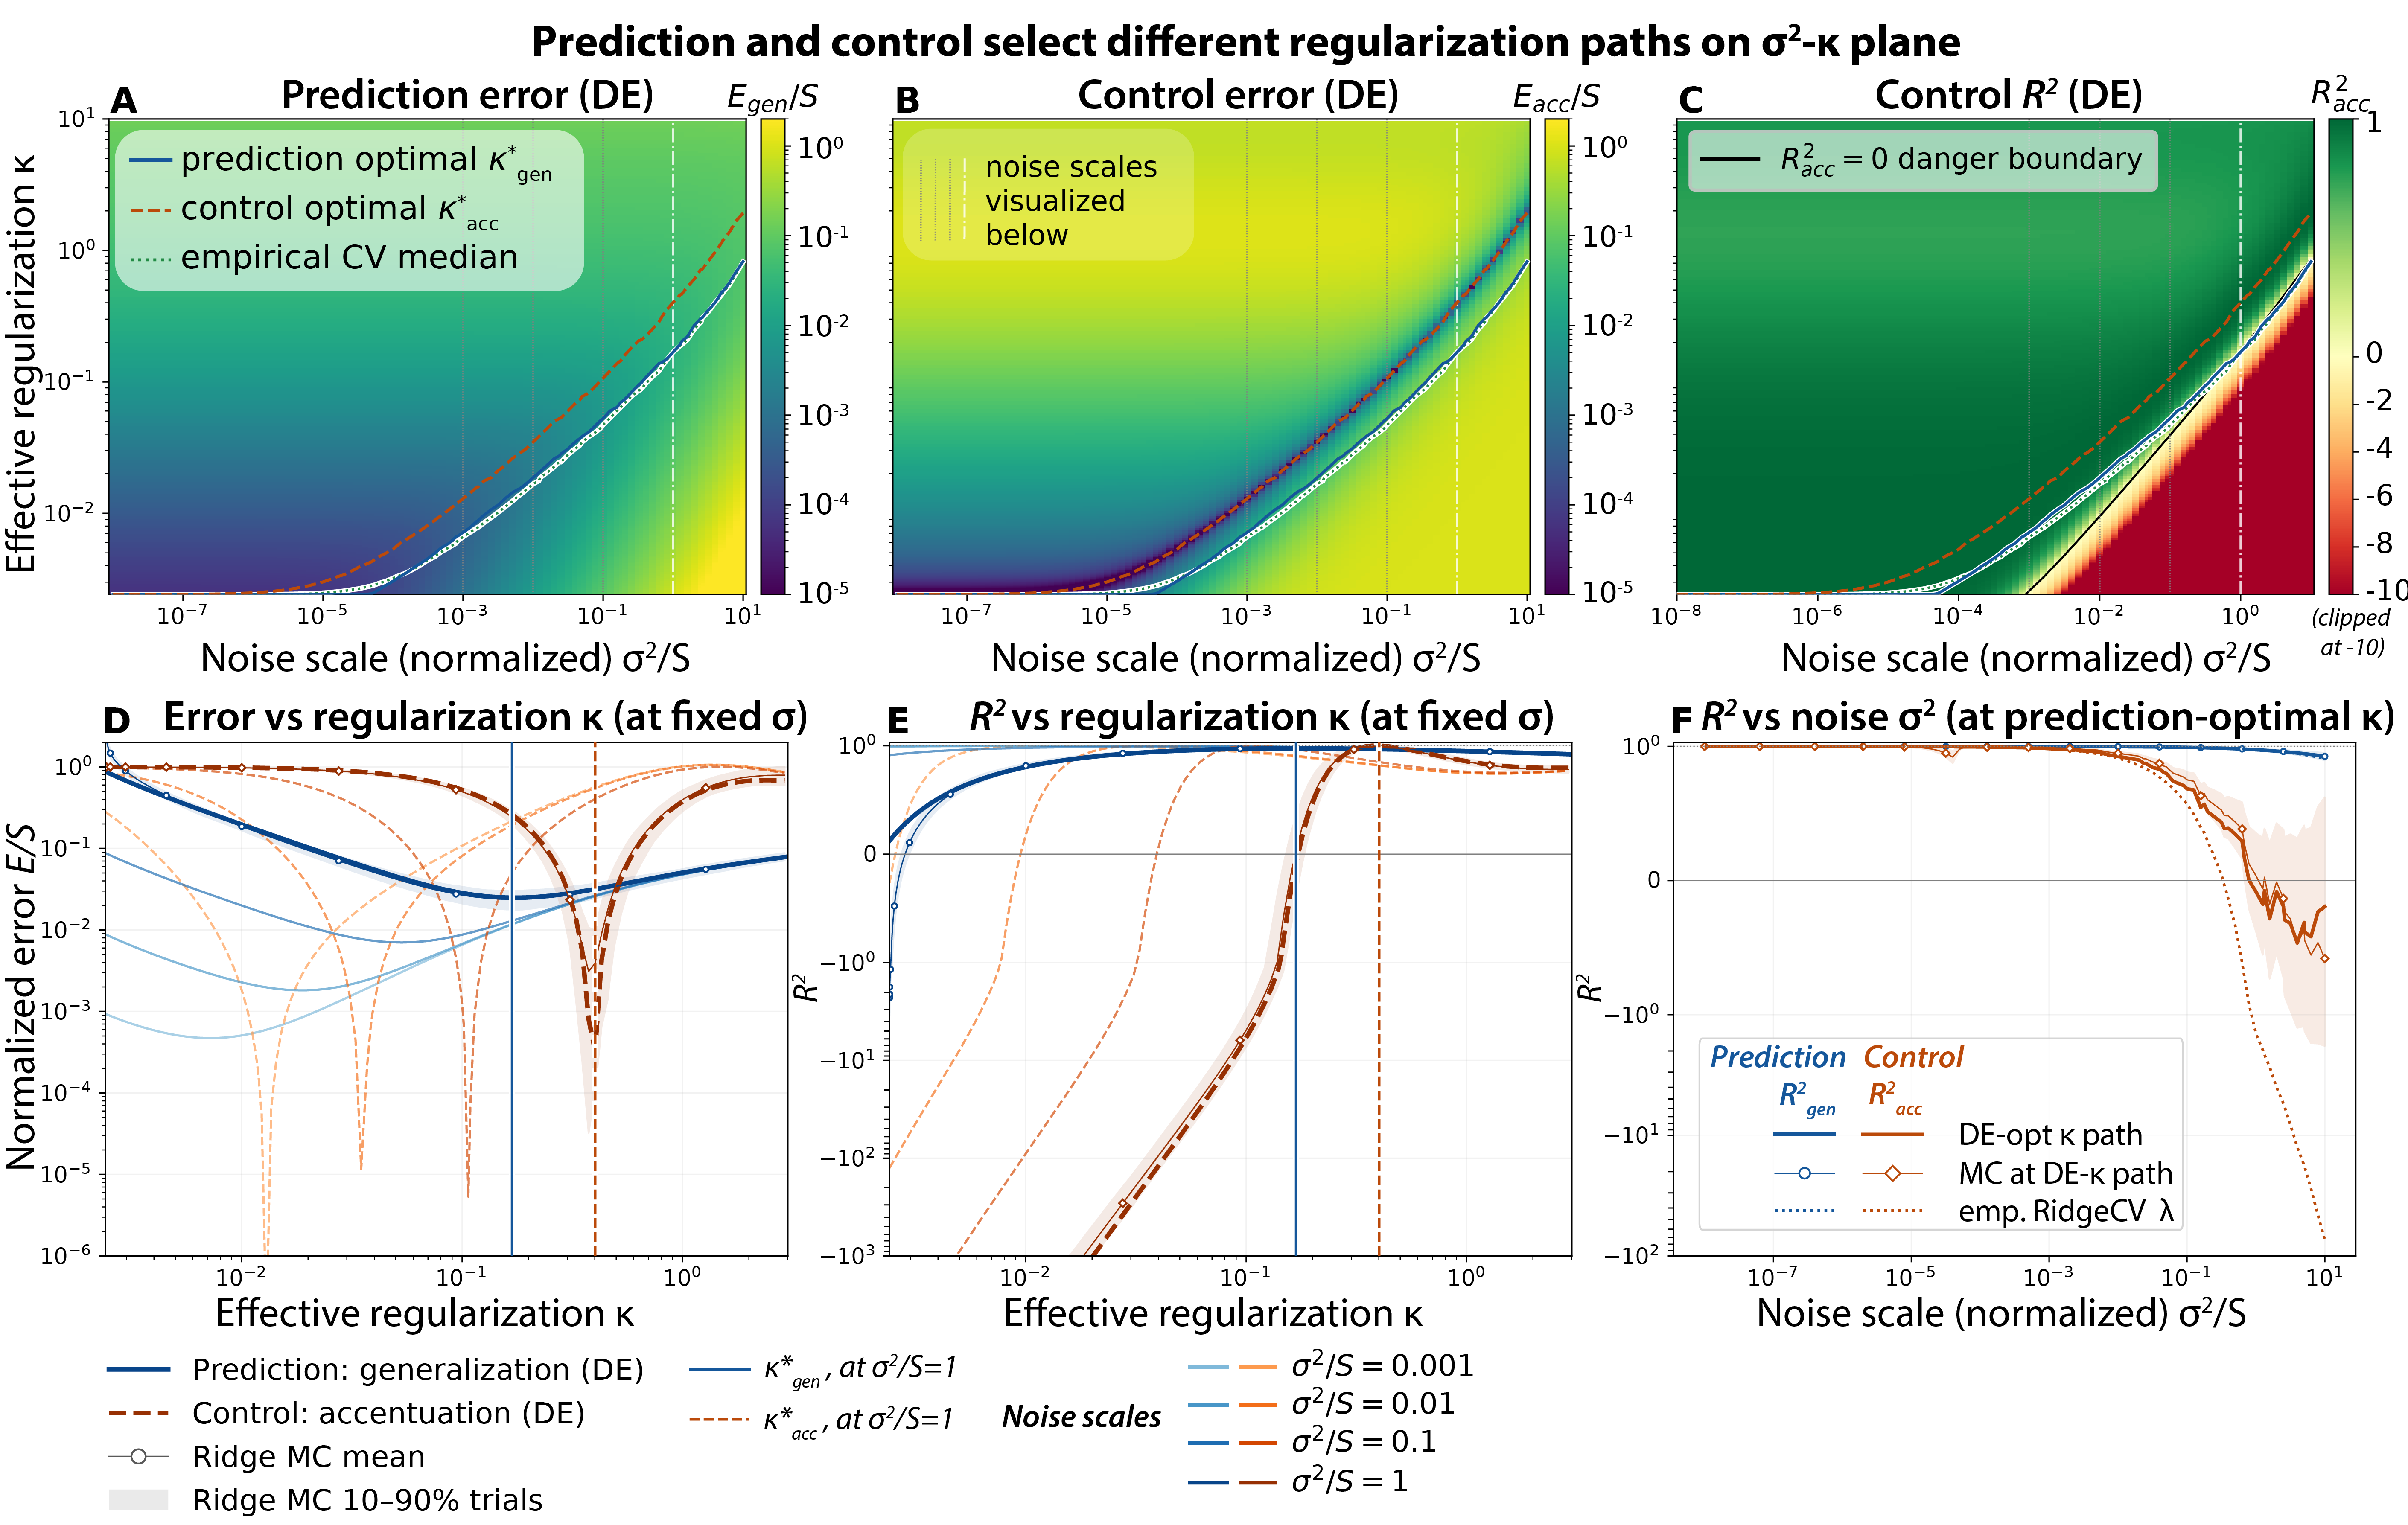
\includegraphics[width=0.5\linewidth,height=1.45in,keepaspectratio]{figures/Figure_PixRidgeGeometry.png}\hfill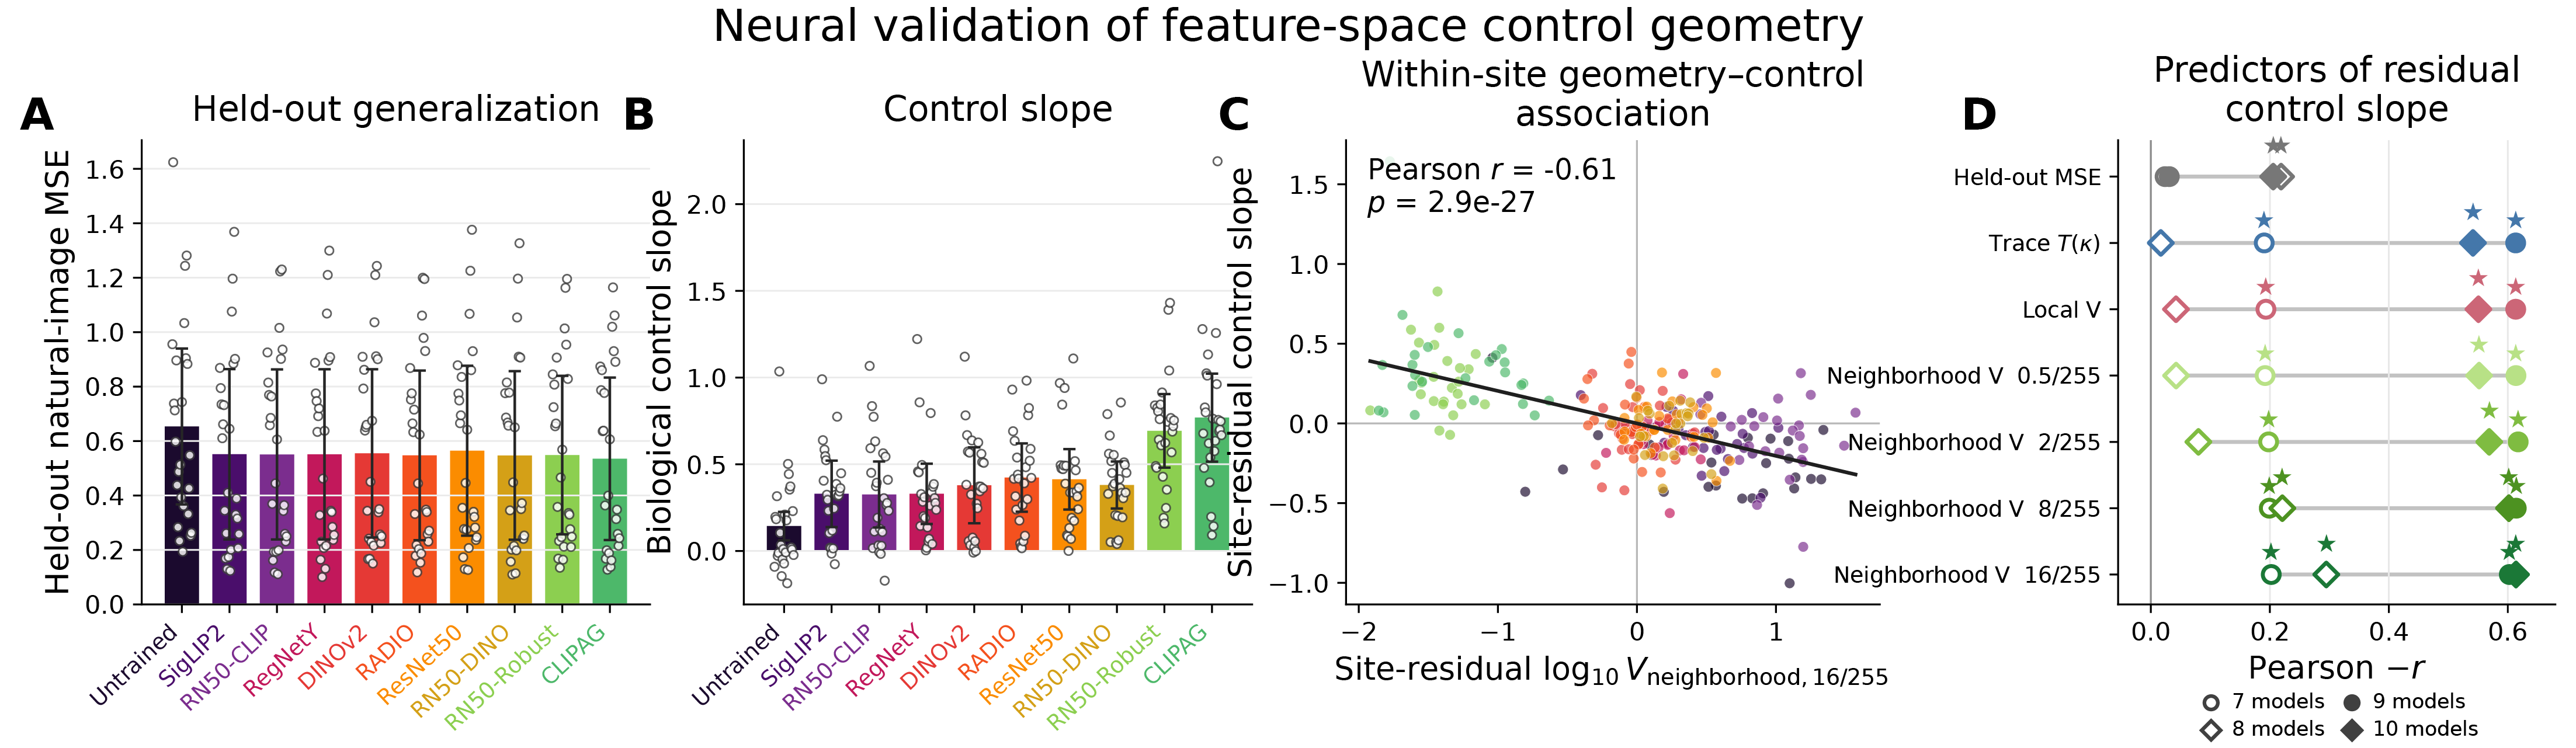
\includegraphics[width=0.48\linewidth,height=1.45in,keepaspectratio]{figures/Figure_nonlinear_neuro_diagnostic.png}}{\textbf{Theory and validation.}
\textbf{A}~Pixel ridge on van Hateren images: $R^2_{\rm gen}$ and $R^2_{\rm acc}$ against the penalty at several noise levels (lines, theory; markers, Monte Carlo).
\textbf{B}~Prediction-preserving rotations of a top-500-PC feature map: $E_{\rm gen}$ and the selected penalty are exactly constant while $R^2_{\rm acc}$ collapses.
\textbf{C}~Neural data of~[1]: site-centred control slope against $\log_{10}T_\phi$ across 250 site--model pairs, and its correlation with held-out error versus $T_\phi$ for subsets of 10, 9, 8 and 7 models.}{fig:theory}

\runsection{Feature maps: why equally predictive models differ.}
Idealize a backbone as a fixed linear map $F\in\R^{p\times d}$, fit $\hat w$ by ridge on $F\x$, and accentuate along the pixel gradient $\bhat=F^\top\hat w$. Prediction sees $F$ only through $\Sigma_F=F\Sigma F^\top$ and $F\Sigma\bstar$; control additionally depends on $FF^\top$ and $F\bstar$. For anisotropic $\Sigma$, the maps $F\mapsto F\Sigma^{1/2}Q\Sigma^{-1/2}$, with $Q$ orthogonal and fixing $\Sigma^{1/2}\bstar$, leave $E_{\rm gen}(\kappa)$ and the cross-validated penalty exactly unchanged while changing control at will: along one such path $R^2_{\rm acc}$ falls from near one to $-10^8$ (Fig.~2B). The map enters the norm inflation through a response-independent \emph{gradient-geometry factor},
\begin{equation}\small
V_F=\frac{E_{\rm gen}+\sigma^2}{n}\,T_F,\qquad
T_F(\kappa)=\sum_k\Big(\frac{s_k}{s_k+\kappa}\Big)^2\frac{\|g_k\|^2}{g_k^\top\Sigma g_k},\qquad g_k=F^\top v_k,
\label{eq:TF}
\end{equation}
with $(s_k,v_k)$ the eigenpairs of $\Sigma_F$: a map is fragile when its well-resolved feature directions backpropagate into low-variance, high-spatial-frequency pixel directions, the linear form of (iii).

\runsection{Deep networks and neural validation.}
With the Jacobian $J_\phi(x)$ of a nonlinear feature map in place of $F$, $T_\phi=\sum_k s_k\|J_\phi(x)^\top v_k\|^2/(s_k+\kappa)^2$ needs one backward pass per feature PC. Across the 250 site--model pairs of~[1], after removing each site's mean controllability, held-out error carries no ordering information (Pearson $r=0.02$ with control slope over nine trained models), whereas $T_\phi$ reaches $r=-0.61$ (Fig.~2C); the two adversarially trained models, the strongest controllers, have the smallest $T_\phi$.

\runsection{Significance.}
Prediction measures weight error in the covariance metric, control along the model's own gradient; the high-frequency artifacts of failed accentuations are the signature of directions natural images never constrained. Selecting encoding models by held-out prediction, as benchmarks do, cannot certify them for gradient-based control~[5]; validation must constrain the gradient, e.g.\ through $T_\phi$, or test generated stimuli directly.

% ---------------------------------------------------------------- references (10 pt, run-in, hand-written; numbers are hard-coded in the text)
\vspace{3pt}
{\fontsize{10}{10.5}\selectfont\setlength{\parskip}{0pt}\noindent\textbf{References.}
[1] Prince, Wang, et al. (2026). Parametric neural control differentiates top neural network models of primate visual cortex. \emph{bioRxiv}.
[2] Hamblin et al. (2024). Feature accentuation. \emph{arXiv:2402.10039}.
[3] Dobriban \& Wager (2018). High-dimensional asymptotics of prediction. \emph{Ann.\ Stat.}\ 46:247--279.
[4] Hastie et al. (2022). Surprises in high-dimensional ridgeless least squares interpolation. \emph{Ann.\ Stat.}\ 50:949--986.
[5] Bashivan, Kar \& DiCarlo (2019). Neural population control via deep image synthesis. \emph{Science} 364:eaav9436.\par}
\end{document}
